% Study deck: separable NM-ROM — architecture, training, and why linear problems
% are quadrature-free while nonlinear ones are sampled.
% Numbers are copied from reports/2026-08-28-presentation-notes.md, whose tables
% are generated from the run JSONs by gen_2026-08-27-b1d-nodes-and-poisson-qf.py.
% Build: latexmk -pdf 2026-08-29-study-deck-linear-vs-nonlinear-residuals.tex
\documentclass[10pt,aspectratio=169]{beamer}
\usetheme{default}
\usecolortheme{default}
\setbeamertemplate{navigation symbols}{}
\setbeamertemplate{footline}[frame number]
\setbeamertemplate{itemize items}[circle]
\setbeamertemplate{blocks}[rounded][shadow=false]
\usepackage{amsmath,amssymb,bm}
\usepackage{booktabs}
\usepackage{tikz}
\usetikzlibrary{arrows.meta,positioning,fit,calc}
\usepackage{graphicx}
\usepackage{xcolor}

% --- palette (roles) ---
\definecolor{trained}{HTML}{C6531C}   % orange: trained by gradient
\definecolor{trainedbg}{HTML}{FBE9E0}
\definecolor{frozen}{HTML}{2F5F8F}    % blue: frozen / precomputed
\definecolor{frozenbg}{HTML}{E2ECF6}
\definecolor{solved}{HTML}{237A58}    % green: solved by a convex fit
\definecolor{solvedbg}{HTML}{DFF0E7}
\definecolor{plainbg}{HTML}{F7F7F2}
\definecolor{ink}{HTML}{152028}
\definecolor{accent}{HTML}{2F5F8F}

\setbeamercolor{structure}{fg=accent}
\setbeamercolor{title}{fg=ink}
\setbeamercolor{frametitle}{fg=ink}
\setbeamercolor{block title}{bg=frozenbg,fg=ink}
\setbeamercolor{block body}{bg=plainbg,fg=ink}
\setbeamercolor{block title alerted}{bg=trainedbg,fg=ink}
\setbeamercolor{block body alerted}{bg=plainbg,fg=ink}
\setbeamercolor{block title example}{bg=solvedbg,fg=ink}
\setbeamercolor{block body example}{bg=plainbg,fg=ink}
\setbeamerfont{frametitle}{series=\bfseries,size=\large}
\setbeamersize{text margin left=6mm,text margin right=6mm}
\AtBeginDocument{\setlength{\abovedisplayskip}{4pt}\setlength{\belowdisplayskip}{4pt}\setlength{\abovedisplayshortskip}{2pt}\setlength{\belowdisplayshortskip}{2pt}}
\setbeamertemplate{frametitle}{\vspace{2mm}\insertframetitle\par\vspace{1mm}}

\tikzset{
  box/.style={draw, rounded corners=2pt, align=center, font=\scriptsize, inner sep=4pt, minimum height=8mm},
  tr/.style={box, fill=trainedbg, draw=trained},
  fz/.style={box, fill=frozenbg, draw=frozen},
  sv/.style={box, fill=solvedbg, draw=solved},
  pl/.style={box, fill=plainbg, draw=gray!70},
  arr/.style={-{Stealth[length=2mm]}, thick, color=gray!60!black},
}

\newcommand{\T}{^{\top}}
\newcommand{\R}{\mathbb{R}}

\title{Separable NM-ROM: architecture, training,\\ and why linear problems need no quadrature}
\subtitle{A study deck --- what is learned, what is frozen, what is exact, what is sampled}
\author{Tunable-NM-ROM project}
\date{29 August 2026}

\begin{document}

\begin{frame}
  \titlepage
  \begin{center}\scriptsize
    Numbers: single-seed, f64, gate-checked A100 runs; tables reproduced from the generated presentation notes (28 Aug 2026).
  \end{center}
\end{frame}

% -------------------------------------------------------------------
\begin{frame}{The question this deck answers}
  \begin{columns}[T]
    \column{0.5\textwidth}
    \begin{block}{The setup}
      A PDE solution $u(x)$ on a fine grid ($n$ up to $2.6\times10^{5}$ points) is represented by a
      \textbf{small latent vector} $z\in\R^{K}$ ($K=8$ or $16$) through a \textbf{decoder}.\\[2pt]
      The reduced-order model (ROM) solves the PDE \emph{for $z$}, never for the grid values directly.
    \end{block}
    \begin{block}{The catch}
      The PDE residual is a \emph{sum over the whole grid}. If every solver iteration had to decode
      the field on the grid and sum it, the ROM would cost as much as the full solver.
    \end{block}
    \column{0.5\textwidth}
    \begin{alertblock}{What we will see}
      \begin{enumerate}
        \item How the decoder is built so the grid can be \emph{factored out}.
        \item How it is trained (stage 1), then frozen.
        \item \textbf{Linear PDE (Poisson):} the whole residual collapses to a small precomputed table --- \emph{no sampling, no decoding, exact}.
        \item \textbf{Nonlinear PDE (Burgers):} one term refuses to collapse --- we \emph{sample} it at a few points and \emph{learn where} (stage 2).
      \end{enumerate}
    \end{alertblock}
  \end{columns}
\end{frame}

% -------------------------------------------------------------------
\section{Architecture}
\begin{frame}{The separable decoder}
  \[
    u(x;z) \;=\; bc(x)\,\big\langle\, g(x),\; h(z)\,\big\rangle
    \;=\; bc(x)\sum_{j=1}^{R} g_j(x)\,h_j(z)
  \]
  \begin{columns}[T]
    \column{0.48\textwidth}
    \begin{itemize}
      \item $g(x)\in\R^{R}$ --- the \textbf{bank}: $R$ spatial \emph{shapes} (Fourier features $\to$ small MLP). Depends on $x$ only.
      \item $h(z)\in\R^{R}$ --- the \textbf{head}: MLP + linear skip from the latent to $R$ \emph{mixing amounts}. Depends on $z$ only.
      \item $bc(x)$ --- a fixed mask that makes the boundary condition hold exactly.
      \item $R=32$ (Burgers), $R=64$--$96$ (Poisson).
    \end{itemize}
    \column{0.52\textwidth}
    \begin{block}{Why ``separable'' matters}
      The two tracks never see each other's input. Evaluate the bank on any point set once and store it as a table
      \[
        G \in \R^{n\times R},\qquad G_{ij} = bc(x_i)\,g_j(x_i).
      \]
      Then the field on that point set is just
      \[
        u(z) \;=\; G\,h(z) \qquad(\text{table}\times\text{coefficient vector}).
      \]
      \textbf{The field is a mix of $R$ fixed shapes; only the $R$ mixing amounts depend on $z$.}
      Everything downstream exploits exactly this.
    \end{block}
  \end{columns}
\end{frame}

\begin{frame}{Architecture diagram --- who is trained, who is frozen, who is solved}
  \centering
  \resizebox{!}{0.72\textheight}{%
  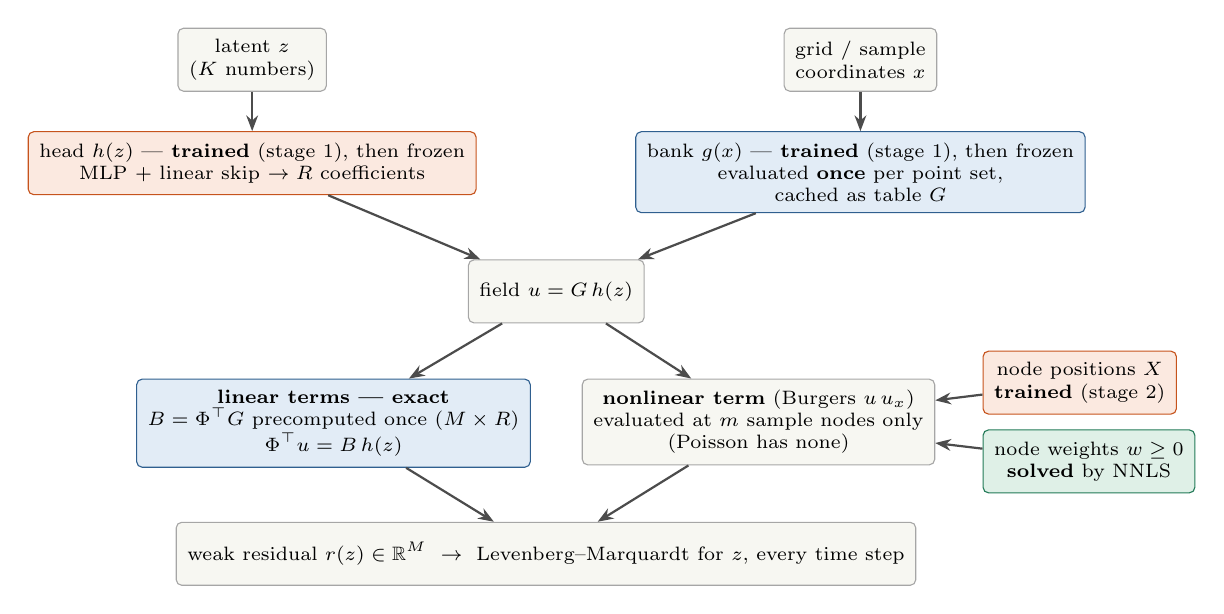
\begin{tikzpicture}[node distance=5mm and 9mm]
    \node[pl] (z) {latent $z$\\($K$ numbers)};
    \node[pl, right=58mm of z] (x) {grid / sample\\coordinates $x$};
    \node[tr, below=of z] (H) {head $h(z)$ --- \textbf{trained} (stage 1), then frozen\\MLP + linear skip $\to R$ coefficients};
    \node[fz, below=of x] (G) {bank $g(x)$ --- \textbf{trained} (stage 1), then frozen\\evaluated \textbf{once} per point set,\\cached as table $G$};
    \node[pl, below=7mm of $(H.south)!0.5!(G.south)$] (U) {field $u = G\,h(z)$};
    \node[fz, below left=7mm and -8mm of U] (LIN) {\textbf{linear terms --- exact}\\$B=\Phi\T G$ precomputed once ($M\times R$)\\$\Phi\T u = B\,h(z)$};
    \node[pl, below right=7mm and -8mm of U] (ADV) {\textbf{nonlinear term} (Burgers $u\,u_x$)\\evaluated at $m$ sample nodes only\\(Poisson has none)};
    \node[tr, right=6mm of ADV, yshift=5mm] (X) {node positions $X$\\\textbf{trained} (stage 2)};
    \node[sv, right=6mm of ADV, yshift=-5mm] (W) {node weights $w\ge0$\\\textbf{solved} by NNLS};
    \node[pl, below=7mm of $(LIN.south)!0.5!(ADV.south)$] (Rr) {weak residual $r(z)\in\R^{M}$ $\;\to\;$ Levenberg--Marquardt for $z$, every time step};
    \draw[arr] (z) -- (H); \draw[arr] (x) -- (G);
    \draw[arr] (H) -- (U); \draw[arr] (G) -- (U);
    \draw[arr] (U) -- (LIN); \draw[arr] (U) -- (ADV);
    \draw[arr] (X) -- (ADV); \draw[arr] (W) -- (ADV);
    \draw[arr] (LIN) -- (Rr); \draw[arr] (ADV) -- (Rr);
  \end{tikzpicture}}

  \vspace{2mm}
  {\scriptsize \textcolor{trained}{$\blacksquare$} trained by gradient \quad
   \textcolor{frozen}{$\blacksquare$} frozen / precomputed (exact path) \quad
   \textcolor{solved}{$\blacksquare$} solved by a convex fit, never gradient-trained}
\end{frame}

% -------------------------------------------------------------------
\section{Training}
\begin{frame}{Stage 1 --- training the decoder (auto-decoder)}
  \[
    L_1 \;=\; \underbrace{\frac{\operatorname{mean}_s\,\|G\,h(z_s)-u_s\|^2}{\operatorname{mean}\,\|u\|^2}}_{\text{relative reconstruction}}
    \;+\; \lambda_{\mathrm{orth}}\,\underbrace{\Big\|\tfrac{G\T G}{n\,s^{2}}-I\Big\|_F^{2}}_{\text{keep the bank well-conditioned}}
  \]
  \footnotesize
  \begin{columns}[T]
    \column{0.55\textwidth}
    Jointly optimise the bank $g$, the head $h$, and \textbf{one latent code $z_s$ per training snapshot $u_s$}
    (there is no encoder --- the codes are free variables). $\lambda_{\mathrm{orth}}=10^{-4}$; Adam, full batch, warm-up then cosine decay ($10^{-3}\to10^{-5}$), 40\,000 steps.
    \column{0.45\textwidth}
    \begin{block}{In words}
      \begin{itemize}
        \item First term: ``every training snapshot must be reconstructible from \emph{some} 8-number code.''
        \item Second term: ``the $R$ shapes should be roughly orthogonal'' --- a conditioning nudge so the mixing amounts stay well-scaled; it does not change what the decoder can represent.
      \end{itemize}
    \end{block}
    \begin{alertblock}{After stage 1}
      Bank, head, and codes are \textbf{frozen}. Nothing downstream ever changes the decoder.
      The training codes are discarded; the solver finds its own $z$ at run time.
    \end{alertblock}
  \end{columns}
\end{frame}

\begin{frame}{How the decoder is used online --- it defines a manifold, it does not predict}
  \footnotesize
  \begin{columns}[T]
    \column{0.5\textwidth}
    \textbf{Weak form.} Pick $M$ test functions $\Phi\in\R^{n\times M}$ (sine modes = exact eigenvectors of the discrete Laplacian, $\Delta\Phi = \Phi\,\Lambda$). The residual handed to the solver is the PDE residual projected onto them:
    \[
      r(z) \;=\; \Phi\T\,\mathcal{R}\big(G\,h(z)\big)\;\in\R^{M},\qquad M = 32\text{ or }64 .
    \]
    \textbf{Solve.} Each time step: damped Levenberg--Marquardt over the $K$ latent unknowns, driving $r(z)\to0$; needs $r$ and $\partial r/\partial z$.
    \column{0.5\textwidth}
    \begin{block}{The cost question}
      $\Phi\T\mathcal{R}(u)$ is a \textbf{sum over all $n$ grid points}. Done naively, each of thousands of solver iterations would
      \begin{enumerate}
        \item decode $u=G\,h(z)$ on the grid ($n\times R$ flops),
        \item apply the PDE operator on the grid,
        \item sum against $M$ test modes.
      \end{enumerate}
      That is the full-order cost, every iteration.
    \end{block}
    \begin{block}{Two ways out}
      \textbf{Exact:} regroup the arithmetic so the grid disappears (works when the term is linear).\\
      \textbf{Approximate:} estimate the sum from $m\ll n$ sample points with weights --- \emph{quadrature} (needed when the term is nonlinear).
    \end{block}
  \end{columns}
\end{frame}

% -------------------------------------------------------------------
\section{Linear problems: quadrature-free}
\begin{frame}{Why a linear term needs no sampling}
  \begin{block}{The one fact}
    \centering
    \textbf{A weighted sum of a mix equals the mix of the weighted sums.}
  \end{block}
  \[
    \Phi\T u \;=\; \Phi\T\Big(\sum_j h_j\,G_{:,j}\Big) \;=\; \sum_j h_j\,\big(\Phi\T G_{:,j}\big) \;=\; \underbrace{(\Phi\T G)}_{B\,:\;M\times R}\,h(z)
  \]
  \footnotesize
  \begin{columns}[T]
    \column{0.46\textwidth}
    The field is a mix of $R$ fixed shapes, $u = \sum_j h_j(z)\,G_{:,j}$, and a linear residual term is a fixed weighted sum of the field --- hence the line above.
    $B$ does not depend on $z$ $\Rightarrow$ compute it \textbf{once}, offline, on the full grid. Online: an $M\times R$ matrix times $R$ numbers.\\[4pt]
    \textbf{Exact, not approximate.} Nothing was estimated; it is the same arithmetic regrouped: $\Phi\T(G\,h)=(\Phi\T G)\,h$.
    \column{0.54\textwidth}
    \begin{exampleblock}{Shopping analogy}
      Every cart is a mix of the same 32 products in different amounts. You do not re-price the cart item by item each time; you look up 32 unit prices once, and the total is amounts $\times$ unit prices.
      $B$ is the unit-price sheet: for each of $M$ test modes and each of $R$ shapes, ``what this shape contributes to this mode.'' $64\times32 = 2\,048$ numbers, computed once.
    \end{exampleblock}
  \end{columns}
\end{frame}

\begin{frame}{Poisson: the whole residual is a small table}
  \[
    \boxed{\;r(z) \;=\; W\odot\big[\,\Lambda\,B\,h(z) \;-\; f_M\,\big]\;}\qquad
    \frac{\partial r}{\partial z} \;=\; W\odot\Lambda\,B\;\frac{\partial h}{\partial z},\qquad B=\Phi\T G,\quad f_M=\Phi\T f
  \]
  \footnotesize
  \begin{columns}[T]
    \column{0.52\textwidth}
    Poisson: $-\Delta u = f$. Every term is linear in $u$.
    \begin{itemize}
      \item \textbf{Laplacian moved onto the test modes.} Because $\Delta\Phi=\Phi\Lambda$,
        $\;\Phi\T(\Delta u) = (\Delta\Phi)\T u = \Lambda\,\Phi\T u.$
        The operator becomes $M$ known numbers $\Lambda$ --- it never touches the field.
      \item \textbf{Source term} projected once: $f_M=\Phi\T f$.
      \item $\partial h/\partial z$: autodiff of an $8\!\to\!32$ MLP.
      \item $W$: fixed per-mode scaling that balances the rows.
    \end{itemize}
    \column{0.48\textwidth}
    \begin{block}{What runs online}
      \begin{itemize}
        \item the tiny head $h(z)$,
        \item a $64\times32$ matvec,
        \item the head's $32\times8$ Jacobian.
      \end{itemize}
      \textbf{No grid. No decode. No sample points. No fitted weights.}
      The field $G\,h(z)$ is formed once, at the very end, to write out the answer.
    \end{block}
    \begin{block}{What ``0 sample points'' means}
      The sampled (NNLS) path estimates the same $M$ numbers from 256 chosen points --- and gets them 5--8\,\% wrong at solutions. The quadrature-free path computes them exactly and does not need the points at all.
    \end{block}
  \end{columns}
\end{frame}

\begin{frame}{Poisson 2D results ($N=128/256/512$, same solver, same frozen decoders)}
  \centering\scriptsize
  \begin{tabular}{@{}rlrrrrrr@{}}
    \toprule
    $N$ & path & sample pts & solve ms & solution err & resid.\ err vs full & grad.\ cos (min) & setup s\\
    \midrule
    128 & full grid & 15\,876 & 3.98 & 3.06e-2 & 0 (ref) & 1.000 & --- \\
    128 & sampled (NNLS) & 256 & 3.14 & 3.06e-2 & 7.9e-2 & $-0.61$ & 28.6 \\
    128 & \textbf{quadrature-free} & \textbf{0} & \textbf{2.93} & 3.06e-2 & \textbf{4.2e-14} & \textbf{1.000} & \textbf{0.9} \\
    \midrule
    256 & full grid & 64\,516 & 4.96 & 3.14e-2 & 0 & 1.000 & --- \\
    256 & sampled (NNLS) & 256 & 2.75 & 3.14e-2 & 6.2e-2 & $-0.60$ & 37.3 \\
    256 & \textbf{quadrature-free} & \textbf{0} & \textbf{2.68} & 3.14e-2 & \textbf{3.6e-14} & \textbf{1.000} & \textbf{0.7} \\
    \midrule
    512 & full grid & 260\,100 & 11.11 & 3.15e-2 & 0 & 1.000 & --- \\
    512 & sampled (NNLS) & 256 & 3.09 & 3.15e-2 & 5.5e-2 & $-0.65$ & 25.4 \\
    512 & \textbf{quadrature-free} & \textbf{0} & \textbf{2.87} & 3.15e-2 & \textbf{3.3e-14} & \textbf{1.000} & \textbf{0.8} \\
    \bottomrule
  \end{tabular}

  \vspace{3mm}
  \begin{columns}[T]
    \column{0.33\textwidth}\small
    \textbf{Exact:} residual matches the full grid to $\sim$13 digits at every solver solution (zero gate failures).
    \column{0.33\textwidth}\small
    \textbf{Fastest and flat in $N$:} full grid grows 4$\to$11 ms; quadrature-free stays $\sim$2.9 ms.
    \column{0.33\textwidth}\small
    \textbf{Nothing to fit:} the 25--37 s NNLS quadrature fit disappears; the sampled rule's gradient could even point the wrong way ($\cos<0$).
  \end{columns}
\end{frame}

% -------------------------------------------------------------------
\section{Nonlinear problems: sampled}
\begin{frame}{Why a nonlinear term breaks the trick}
  Burgers: $u_t + u\,u_x = \nu\,u_{xx}$. The advection term multiplies the field by itself:
  \[
    \Phi\T\big(u\odot u_x\big)
    \;=\; \Phi\T\Big[\Big(\sum_j h_j G_{:,j}\Big)\odot\Big(\sum_k h_k G'_{:,k}\Big)\Big]
    \;=\; \sum_{j,k} h_j\,h_k\;\Phi\T\big(G_{:,j}\odot G'_{:,k}\big)
  \]
  \footnotesize
  \begin{columns}[T]
    \column{0.5\textwidth}
    \begin{itemize}
      \item Mixing does not pass through a product: every \emph{pair} of shapes appears ($R^2$ terms, $M\times R\times R$ table).
      \item Worse: our discretisation is \textbf{sign-upwind} --- the stencil for $u_x$ switches with the sign of $u$ at each point. That is not a polynomial in $h$; no table can hold it.
    \end{itemize}
    \column{0.5\textwidth}
    \begin{alertblock}{Consequence}
      The only way to know the term's value is to \textbf{actually look at the field somewhere}.
      So we must decode at \emph{some} points --- and then we have to choose \emph{which} points and \emph{what weights}: that is quadrature, and its error enters the ROM's error.
    \end{alertblock}
    \begin{block}{But only that one term}
      Time derivative and diffusion are linear $\Rightarrow$ they still go through $B=\Phi\T G$, exactly (``exlin''). Sampling touches the advection term and nothing else.
    \end{block}
  \end{columns}
\end{frame}

\begin{frame}{What we do for Burgers: exact linear terms + sampled advection}
  \small Backward-Euler step from $z^n$ to $z$; $N(u)=u\,u_x$ (sign-upwind); $m$ nodes $X$ with weights $w\ge0$; $\Phi_X,G_X$ = test modes and bank evaluated at the nodes:
  \[
    r(z) \;=\; W\odot\Big[\underbrace{B\big(h(z)-h(z^n)\big)}_{\text{time derivative, exact}}
    \;+\;\Delta t\Big(\underbrace{\Phi_X\T\big(w\odot N_X(G_X h(z))\big)}_{\text{advection, sampled at } m \text{ nodes}}
    \;+\;\underbrace{\nu\,\Lambda\,B\,h(z)}_{\text{diffusion, exact}}\Big)\Big]
  \]
  \begin{columns}[T]
    \column{0.5\textwidth}
    \begin{block}{The per-iteration cost}
      Decode at $m$ nodes only ($m\times R$), one upwind stencil on $m$ values, an $M\times m$ matvec, and the exact linear part. \textbf{Independent of the grid size $n$.} Measured: latent solve flat from $N=128$ to $4096$.
    \end{block}
    \column{0.5\textwidth}
    \begin{exampleblock}{Choosing the nodes: baseline = NNLS}
      Given positions $X$, weights are fit by non-negative least squares so the sampled term reproduces the exact full-grid term on training states. Convex, no gradients, always available as a fallback. Positions themselves are the free choice --- stage 2 learns them.
    \end{exampleblock}
  \end{columns}
\end{frame}

\begin{frame}{Stage 2 --- learning where to sample (decoder frozen)}
  \small Only the node positions $X$ are trainable. The loss is a \textbf{mismatch against the exact full-grid term}, in value \emph{and} in the $z$-gradient the solver follows:
  \[
    L_{\mathrm{samp}} = \operatorname{mean}_s
      \frac{\big\|W_s\big(\Phi_X\T(w\odot N_X(u_s)) - \Phi\T N(u_s)\big)\big\|^2}{\|W_s\,\Phi\T N(u_s)\|^2},
    \qquad L_{\mathrm{jac}} = \text{same expression for }\partial_z(\cdot)
  \]
  \[
    L_2 = \frac{L_{\mathrm{samp}}}{L_{\mathrm{samp}}^{0}} + \frac{L_{\mathrm{jac}}}{L_{\mathrm{jac}}^{0}}
        + w_{\mathrm{sep}}\sum_{i<j}\operatorname{relu}\big(d_{\min}-|x_i-x_j|\big)^2
  \]
  \footnotesize
  \begin{columns}[T]
    \column{0.5\textwidth}
    \begin{block}{Optimisation}
      \begin{itemize}
        \item Adam on $X$ only, LR $3\times10^{-3}$, 2\,000 steps.
        \item A sigmoid box keeps every node inside the domain.
        \item The last term keeps nodes apart (minimum separation).
        \item Each term $\div$ its starting value: both begin at 1, equal weight.
      \end{itemize}
    \end{block}
    \column{0.5\textwidth}
    \begin{exampleblock}{Weights are never gradient-trained}
      Every 500 steps the weights $w\ge0$ are re-solved by NNLS on the same loss rows (variable projection). The convex NNLS rule is therefore always the fallback: learning can only move points, never damage the decoder.
    \end{exampleblock}
  \end{columns}
\end{frame}

\begin{frame}{Stage 2 --- the design choices, and why}
  \begin{columns}[T]
    \column{0.5\textwidth}
    \begin{block}{Teacher frozen}
      The full-grid advection term and the decoder cannot move, so the loss cannot be gamed by ``fooling the points'' --- only better placement lowers it. (An earlier co-training variant that let the decoder move was negative.)
    \end{block}
    \begin{block}{Match the gradient, not just the value}
      The solver steps along $\partial r/\partial z$. A rule that matches residual values but not their $z$-sensitivity can send the solver the wrong way --- Poisson's NNLS rule had gradient cosines below zero.
    \end{block}
    \column{0.5\textwidth}
    \begin{block}{Held-out states}
      A disjoint set of training states sits in no gradient step and no NNLS row; it monitors whether the placement generalises rather than memorises.
    \end{block}
    \begin{block}{What the certification is}
      Rollouts on 8 fresh test trajectories the decoder never saw, graded against the full-order truth, compared to the same-budget NNLS rule and to the full-grid oracle.
    \end{block}
  \end{columns}
\end{frame}

\begin{frame}{1D Burgers results ($N=128\ldots4096$, 8 fresh trajectories, 50 implicit steps)}
  \centering\scriptsize
  \begin{tabular}{@{}rrrrlrl@{}}
    \toprule
    $N$ & decoder floor & oracle & NNLS 32 & learned 32 (vs NNLS) & NNLS 16 & learned 16 (vs NNLS)\\
    \midrule
    128  & 3.71e-3 & 5.01e-3 & 5.48e-3 & 5.02e-3 ($-8.4\%$) & 2.10e-2 & 1.01e-2 (\textbf{$-52\%$})\\
    256  & 3.73e-3 & 6.17e-3 & 6.24e-3 & 6.20e-3 ($-0.6\%$) & 2.56e-2 & 1.07e-2 (\textbf{$-58\%$})\\
    512  & 3.80e-3 & 4.88e-3 & 5.19e-3 & 4.89e-3 ($-5.9\%$) & 2.68e-2 & 1.03e-2 (\textbf{$-62\%$})\\
    1024 & 3.79e-3 & 5.54e-3 & 5.62e-3 & 5.45e-3 ($-2.9\%$) & 2.22e-2 & 8.61e-3 (\textbf{$-61\%$})\\
    2048 & 3.83e-3 & 5.08e-3 & 5.53e-3 & 5.15e-3 ($-7.0\%$) & 2.25e-2 & 8.44e-3 (\textbf{$-63\%$})\\
    4096 & 3.83e-3 & 4.49e-3 & 4.89e-3 & 4.53e-3 ($-7.3\%$) & 2.29e-2 & 9.22e-3 (\textbf{$-60\%$})\\
    \bottomrule
  \end{tabular}

  \vspace{3mm}
  \begin{columns}[T]
    \column{0.33\textwidth}\small
    \textbf{Oracle} = advection summed on the full grid (no sampling): the best any node set can do with this decoder. Flat across $32\times$ in resolution.
    \column{0.33\textwidth}\small
    \textbf{32 nodes:} sampling costs 2--10\,\% over the oracle; learned nodes close 84--97\,\% of that gap --- they land on the oracle.
    \column{0.33\textwidth}\small
    \textbf{16 nodes (starved):} NNLS is 4--5$\times$ the oracle error; learned placement cuts it by 52--63\,\%, six for six. It improves a budget; it does not replace a bigger one.
  \end{columns}
\end{frame}

\begin{frame}{Error over the rollout ($N=512$)}
  \begin{columns}[T]
    \column{0.6\textwidth}
    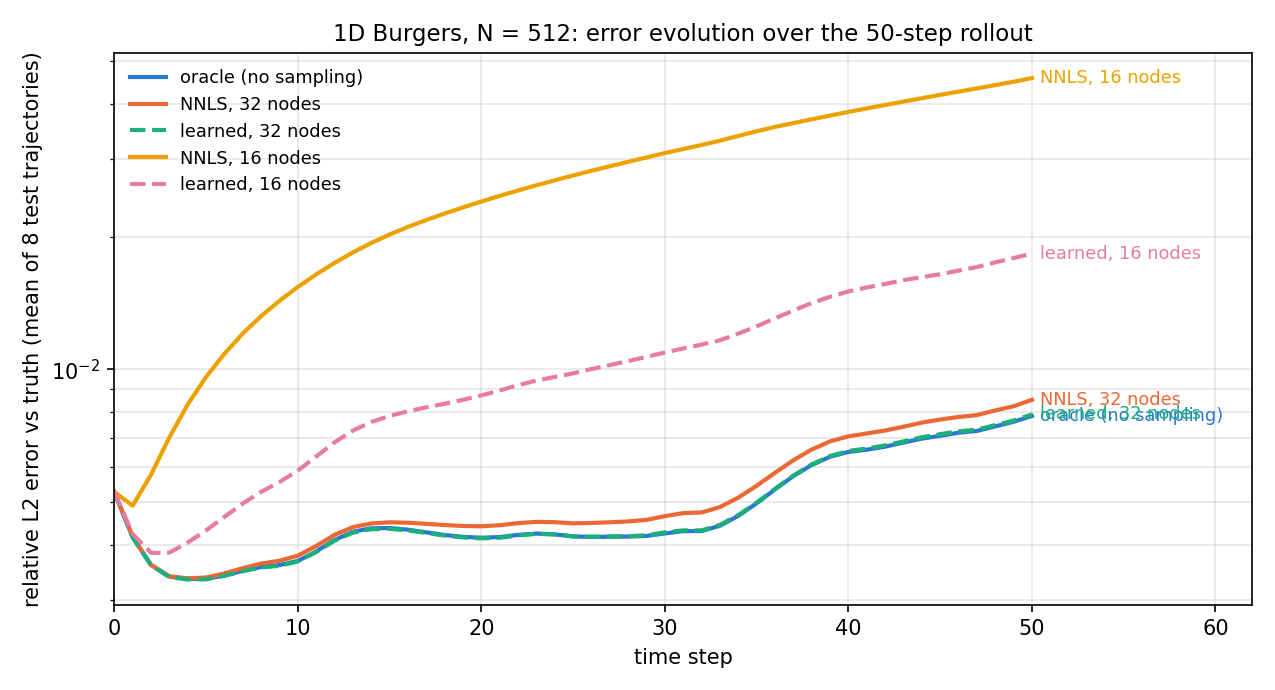
\includegraphics[width=\textwidth]{figs/b1d-error-vs-time-n512.png}
    \column{0.4\textwidth}
    \begin{itemize}
      \item All arms share the same initial-condition fit (step 0).
      \item Oracle and learned-32 are indistinguishable step for step.
      \item The starved NNLS rule (16 nodes) drifts from step 1 onward (4.6e-2 by step 50); learned nodes at the same budget hold it to 1.8e-2.
    \end{itemize}
    \vspace{2mm}
    {\small ROM online cost per 50-step trajectory (A100), independent of resolution: 49--62 ms; 22--24 ms after inner-loop optimisation with errors unchanged to $10^{-9}$.}
  \end{columns}
\end{frame}

% -------------------------------------------------------------------
\section{Summary}
\begin{frame}{Linear vs nonlinear, side by side}
  \centering\scriptsize
  \renewcommand{\arraystretch}{1.15}
  \begin{tabular}{@{}p{0.24\textwidth}p{0.36\textwidth}p{0.36\textwidth}@{}}
    \toprule
     & \textbf{Linear (Poisson)} & \textbf{Nonlinear (Burgers)}\\
    \midrule
    Residual in terms of $h(z)$ & $\Lambda B\,h(z)-f_M$: linear in $h$ & linear terms via $B$; advection $u\,u_x$ is quadratic \emph{and} upwind-switched\\
    Can the grid be folded away? & Yes, entirely: $B=\Phi\T G$ once & Only for the linear terms; advection must be evaluated somewhere\\
    Online per iteration & head $h(z)$ + a $64\times32$ matvec & head + decode at $m$ nodes + stencil + $M\times m$ matvec\\
    Sample points & \textbf{0} & $m$ (32 tight, 16 starved, 128 generous)\\
    Approximation error from the residual & none (matches full grid to $10^{-13}$) & quadrature error; reduced by NNLS weights + learned positions\\
    Anything to fit or train after stage 1 & nothing & NNLS weights (convex) + node positions (stage 2 gradient)\\
    Accuracy limit & decoder floor & decoder floor (oracle) $+$ sampling gap\\
    Cost vs grid size & flat & flat (latent solve measured flat $128\to4096$)\\
    \bottomrule
  \end{tabular}
  \vspace{2mm}
  \begin{block}{One sentence}
    \small The decoder is linear in its last stage, so every linear piece of the physics can be pre-projected onto the test modes once; a nonlinear piece cannot, so we sample it at a few points and learn where those points should be.
  \end{block}
\end{frame}

\begin{frame}{Glossary (1/2)}
  \small
  \begin{description}
    \item[Latent $z$] The $K$ numbers ($8$ or $16$) that stand in for a whole field.
    \item[Bank $g$, head $h$] The two halves of the decoder: shapes in space ($g$; table $G$ once evaluated) and mixing amounts from $z$ ($h$).
    \item[Test modes $\Phi$, $M$] The $M$ sine functions the residual is projected onto (weak form); eigenvectors of the discrete Laplacian with eigenvalues $\Lambda$.
    \item[$B=\Phi\T G$] The precomputed $M\times R$ table that turns any linear grid sum into a small matvec.
    \item[Quadrature] Estimating a grid-wide sum from $m$ sample points with weights. \textbf{Quadrature-free} = the sum is computed exactly without points.
    \item[Full grid / oracle] The residual (Poisson) or the advection term (Burgers) summed over every grid point --- the reference the sampled rules try to match.
  \end{description}
\end{frame}

\begin{frame}{Glossary (2/2)}
  \small
  \begin{description}
    \item[NNLS] Non-negative least squares: fits the node weights so the sampled term reproduces the full-grid term on training states; convex, no gradients.
    \item[Learned nodes] Node positions optimised by gradient (stage 2) with the decoder and teacher frozen; weights still by NNLS.
    \item[Tight / starved / generous budget] $m=32$ ($=M$), $16$, $128$ nodes.
    \item[Decoder floor] The error of the best possible latent for each truth snapshot; nothing downstream can beat it.
    \item[Rollout error] Relative $L_2$ error against the full-order truth over the 50 implicit time steps, mean of 8 fresh test trajectories.
    \item[Gate] An in-job numerical identity check (e.g.\ gate Q: quadrature-free residual $=$ full-grid residual to machine precision at every solution).
  \end{description}
\end{frame}

\end{document}
